\chapter{Deseño}

Neste capítulo documentarase o proceso de deseño que se irá formando de xeito incremental nas sucesivas iteracións da metodoloxía Scrum. Comentarase a arquitectura do modelo de datos que vai manexar a aplicación, así como a distribución deses datos na aplicación, o que nos obrigará a falar da interface gráfica de usuario. Despois disto, mergullarémonos no que é o deseño e máis a implementación dos compoñentes da aplicación.

\section{Deseño global}

O proxecto que imos traballar podería terse desenvolvido, atendendo á súa especificación, baixo un único módulo de traballo. É unha aplicación de escritorio, é dicir, non existe a necesidade, por exemplo, de facer un módulo cliente e un módulo servidor, e polo tanto poderíamos crear un único proxecto de nome JDataMotion que contivese toda a lóxica necesaria para ler, interpretar e procesar datos externos, fornecidos polo usuario.

Sen embargo, e a pesar de todo isto, debemos considerar o requisito de deseño RD01, que nos obriga a definir e facilitar ao usuario unha interface de programación, a cal lle permitirá programar e ensamblar os seus propios filtros no proxecto. Ademais da interface, teremos que publicar as clases das que esta depende. Desta forma, decidimos que o máis práctico era crear un segundo proxecto, ao que mencionaremos a partir de aquí como JDataMotion.common.

E seguindo nesta liña, crearase un terceiro módulo que se usará para probar e exemplificar a efectividade da relación entre os outros dous. Este proxecto chamarase JDataMotion.filters.sample e conterá algunhas clases que implementarán a interface de filtro publicada en JDataMotion.common.

O diagrama que ilustra as relacións entre os 3 módulos sería o que se expón na figura \ref{disenhoGlobal}. O módulo (ou subproxecto) JDataMotion.common contén a interface IFilter (ademáis doutras clases das que depende a interface). Tanto o JDataMotion (a aplicación) como o JDataMotion.filters.sample dependen do módulo común, e en concreto o JDataMotion.filters.sample deberá implementar a interface naquelas clases que vaian ser susceptibles de ser importadas en forma de filtro polo JDataMotion.

\begin{figure}
\centering
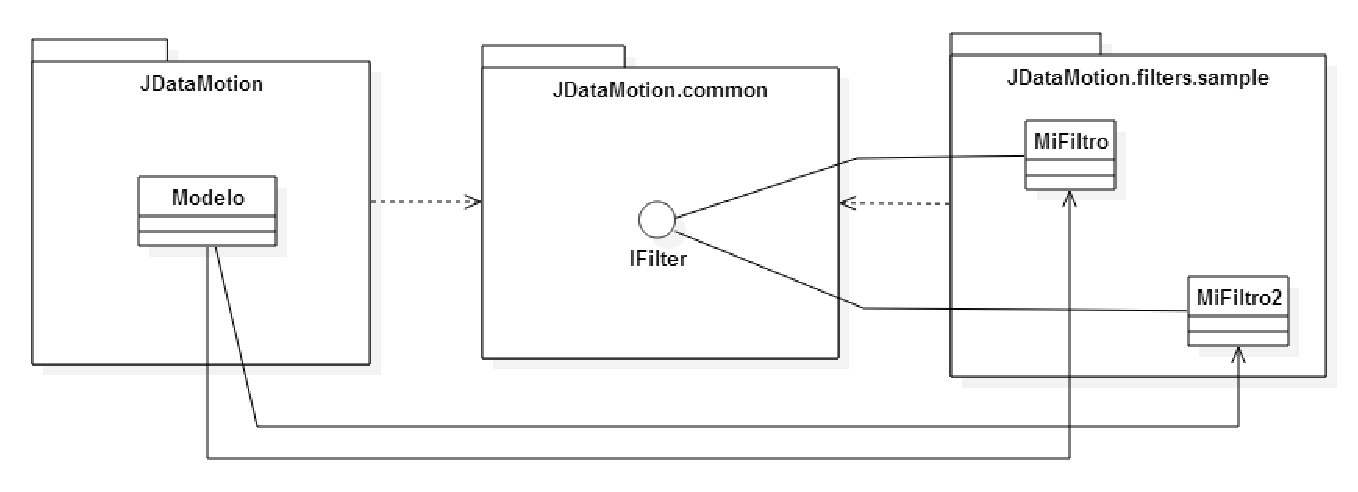
\includegraphics[width=\textwidth,height=\textheight,keepaspectratio]{figuras/disenhoGlobal}
\caption{Deseño global dos 3 módulos que se incluirán dentro do proxecto}
\label{disenhoGlobal}
\end{figure}

A continuación abordaremos o deseño de cada un dos tres módulos implicados neste proxecto.

\section{Deseño de JDataMotion}

Os datos son o punto de partida de todas as funcionalidades deste proxecto. Todo xira arredor do arquivo con información que o usuario importa tras abrir por primeira vez o JDataMotion. O dato debe ser almacenado de xeito adecuado, e accedido só a través dos métodos e clases necesarios, para manter o fluxo de información controlado. A clase que captará, almacenará e distribuirá os datos de cara ás demais clases da aplicación recibirá o nome de Modelo, posto que realmente alberga o modelo da aplicación.

JDataMotion vai ser un programa moi dependente da súa interface de usuario. Os diagramas de dispersión non poden ser visualizados a través dunha simple terminal, e o constante fluxo de datos entre o usuario e o sistema non se pode activar a través dun menú de opcións en termos de usabilidade. Si traballamos co JDataMotion a través dunha interface gráfica multifío como as que Java permite deseñar, a aplicación pode procesar a información ao mesmo tempo que o usuario realiza outras interaccións (ver o modelo, configurar un filtro ou mesmo cancelar a visualización dinámica). Por isto, a clase Vista será un dos artefactos que máis tempo adicaremos a implementar. Vista conterá os ``widgets'' da libraría Swing necesarios para presentar a información ao usuario, e recibir del as novas ordes. Será unha clase complexa e de bastante peso que delegará certas funcións en clases internas ou asociadas.

Só falta unha clase que reciba da Vista as funcionalidades activadas polo usuario e cree un comando que se encargue de realizar o traballo. Esta clase deberá non só disparar o comando, se non que tamén terá que xestionalo, e reaccionar dun xeito específico en caso de que o comando chegue a unha situación de erro. A maioría de comandos influirá directa ou indirectamente sobre o Modelo. A esta clase chamarémoslle Controlador porque a súa responsabilidade será esencialmente esa, a de recibir eventos da Vista e xestionar comandos que actúen de cara ao Modelo. Deste xeito a Vista utilizará a API do Controlador, e quedará exenta de responsabilidade no caso de que se detecten fallas no Modelo.

Acabamos de definir dun xeito explícito cal é o patrón de deseño sobre o que vai xirar toda esta fase do proxecto: o Modelo-Vista-Controlador (MVC). Os patróns de deseño son solucións prácticas a problemas de deseño comúns. En concreto, o Modelo-Vista-Controlador divide o sistema en tres compoñentes coas responsabilidades definidas que xa comentamos anteriormente. A mellor forma de expoñer a aplicación exacta do patrón MVC no noso proxecto é o diagrama da figura \ref{MVC}.

\begin{figure}
\centering
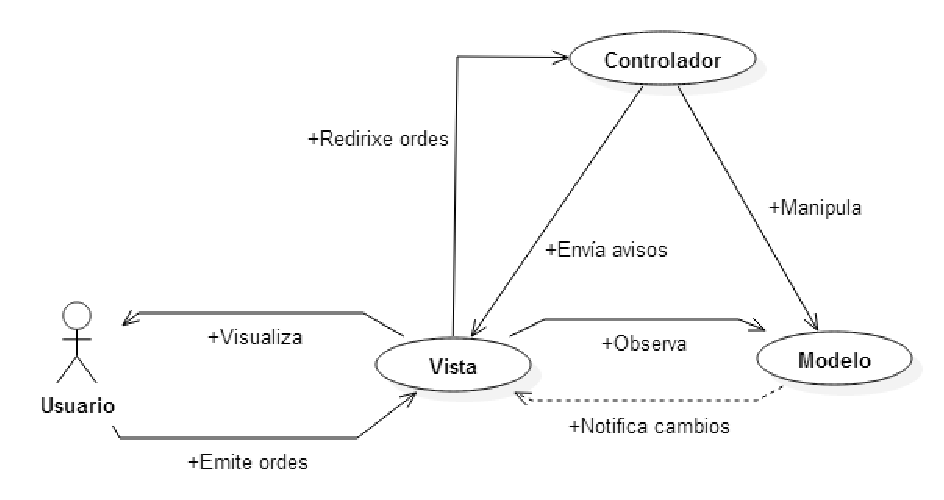
\includegraphics[width=\textwidth,height=\textheight,keepaspectratio]{figuras/MVC}
\caption{Modelo-Vista-Controlador para JDataMotion}
\label{MVC}
\end{figure}

As relacións marcadas cunha liña sólida son asociacións directas (unha clase que actúa de xeito explícito sobre os atributos ou métodos doutra), mentres que a relación marcada cunha liña descontinua representa unha relación indirecta (por exemplo, unha clase que resulta afectada pola actividade doutra). As relacións entre compoñentes detallaranse a continuación.

\begin{itemize}
\item O usuario emite ordes en forma de eventos cara a Vista ao interactuar cos seus botóns e menús.
\item A Vista identifica os eventos que recibe e redirixe cara o Controlador a orde asociada ao evento en cuestión.
\item O Controlador envía un aviso directo á Vista en caso de que a orde que recibe dela levase ao sistema a un estado de erro.
\item O Controlador manipula o Modelo segundo o contido da orde que recibe.
\item O Modelo actúa como entidade observada de cara á Vista. A Vista ten acceso ao Modelo para actualizar a súa aparencia.
\item Do mesmo xeito, que o Modelo sexa observado pola Vista implica que os cambios no modelo serán notificados á Vista, para que esta se actualice no momento do cambio.
\end{itemize} 

Imos documentar máis en profundidade a relación entre a Vista e o Modelo. Comentábamos que a Vista accede ao Modelo para actualizarse cando o desexe, pero ademais o Modelo, cando cambia, notifica á Vista o suceso deste cambio. Temos entón que a Vista actúa como entidade ``observadora'' dun Modelo que é a entidade ``observada''. En esencia, estamos definindo o patrón de deseño Observer.

O patrón de deseño Observer é a mellor resposta que podemos atopar a nivel de deseño para solucionar o problema de manter actualizados ao mesmo nivel o Modelo e a Vista. Se non botásemos man desta solución, teríamos dúas alternativas:

\begin{itemize}
\item Refrescar a vista cada certo intervalo tempo, o cal é ineficiente e seguiría permitindo a posibilidade de que se dese unha incoherencia Vista-Modelo entre refrescos.
\item Permitir ao Modelo que acceda directamente á Vista para invocar un método de actualización, é dicir, asociar directamente a Vista ao Modelo. Isto atenta contra a natureza do Modelo-Vista-Controlador, xa que o Modelo ten que almacenar a información do sistema e abstraerse por completo da Vista ou do módulo que se encargue de representar os seus contidos. Témonos que manter na premisa de que a Vista pode observar ao Modelo e acceder a el para ler datos, pero o Modelo non debe ser consciente da existencia de ningunha Vista.
\end{itemize} 

O patrón Observer pódese aplicar de forma moi sinxela ao noso proxecto. Basta con facer que a Vista implemente a interface \textit{Observer}, de xeito que a obrigue a implementar un método de actualización chamado \textit{update()}, que se disparará cando un obxecto observado cambie o seu estado. Por outra parte, o Modelo só necesita estender a clase \textit{Observable} para ser susceptible de ser observado por un \textit{Observer}. Ao estender esta clase, a Vista xa pode chamar ao método \textit{addObserver(Observer o)} do Modelo, pasándose a ela mesma como parámetro para así incluírse como observadora e ser notificada dos seus cambios.

A asociación dos patróns Modelo-Vista-Controlador e Observer baixo esta forma é bastante común. O libro Pattern-Oriented Software Architecture \cite{pattern-oriented-software-architecture} fai unha boa exposición do que acabamos de mencionar, e aporta o diagrama da figura \ref{MVC-observer} para sintetizar ambos patróns.

\begin{figure}
\centering
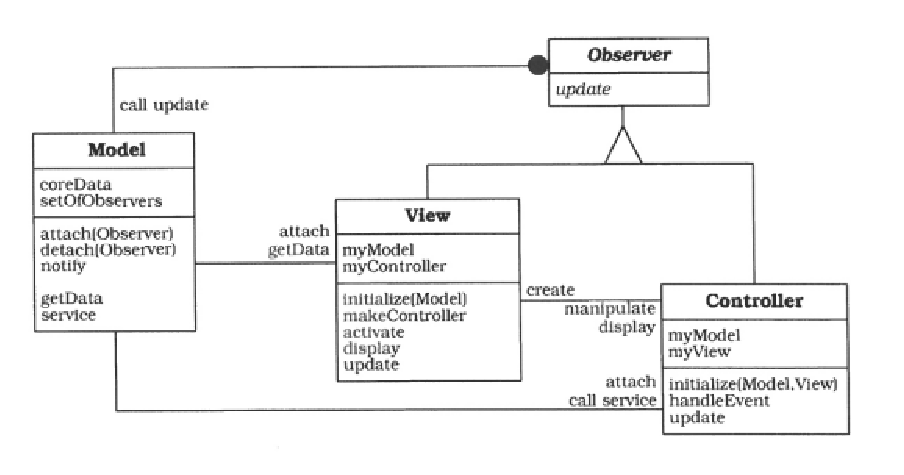
\includegraphics[width=\textwidth,height=\textheight,keepaspectratio]{figuras/MVC-observer}
\caption{Modelo-Vista-Controlador con Observer}
\label{MVC-observer}
\end{figure}

Probablemente a diferencia máis destacable que podemos atopar entre este diagrama e o diagrama que correspondería coa nosa aplicación sería que no noso caso só a Vista implementará a interface \textit{Observer}. O Controlador no noso proxecto non actuará de observador, pois non ten que recibir notificacións ante os cambios do Modelo, xa que de feito el é o responsable directo de todos eses cambios, e non necesita ser notificado de cambios do modelo que non provocase el.

Acabamos de expoñer as 3 clases principais do proxecto e as súas interrelacións, pero debemos ter en conta que cada unha desas clases necesita a axuda doutras que colaboren con ela no obxectivo de cumprir coas súas responsabilidades. O que faremos a continuación será ampliar as 3 entidades básicas do MVC aplicadas ao noso proxecto.

\subsection{Modelo}

O Modelo, como comentábamos, é o responsable de captar e almacenar a información coa que traballamos. A información almacenada clasifícase en 3 conxuntos:

\begin{description}

\item[Instancias:]

Son as tuplas de información coas que se traballa. A estrutura para almacenalas e xestionalas foi reutilizada a partir da API de programación de Weka: a clase Instances. Esta estrutura almacena tanto as propias instancias ou tuplas de información, coma os atributos que levan asociadas. Ademais, contempla toda a información relacionada co atributo: nome, tipo, rango, etc. Esta clase tamén nos facilitará todos os métodos que necesitamos para acceder ou modificar instancias ou atributos. Ademais, a clase Instances de Weka tamén almacena un nome para a relación.

Como veremos, non empregaremos a clase Instances directamente, se non que a estenderemos a través dunha clase á que chamaremos ComparableInstances. A única diferencia entre ambas é que ComparableInstances sobreescribe o método equals(Object o), para determinar que dúas instancias sexan iguais en canto a nome da relación, atributos e tuplas. Isto resultará clave á hora de realizar as probas da aplicación, xa que permitirá verificar que un experimento acada un estado esperado ao aplicarlle unha acción, demostrando a efectividade da mesma.

\item[Filtros:]

O Modelo tamén albergará a secuencia de filtros que utilicemos no noso experimento. Utilizará para isto unha estrutura de tipo lista na que cada novo filtro se engada ao final (se ben é posible cambiar a posición dos filtros e polo tanto a orde da súa aplicación).

Para seren útiles de cara ao Modelo, os filtros deben de conter unha pequena porción de lóxica que a interface IFilter non pode incorporar. Por isto, o Modelo tratará de encapsular cada IFilter co que traballe dentro dun FilterHandler. O FilterHandler só é un manexador da interface que contén, pero con outros campos necesarios como o índice do atributo sobre o que opera o filtro, ou un parámetro de bandeira que indica si o filtro está seleccionado. En canto a métodos, o FilterHandler tamén ofrece ao Modelo un conxunto de procedementos prácticos para traballar co filtro en cuestión.

\item[Outros elementos:]

O Modelo tamén almacena outros datos máis discretos acerca do experimento, como son os índices de atributo temporal e nominal que se empregarán na visualización, a dirección ao ficheiro de orixe e o resumo SHA1 do mesmo (para posibilitar a creación e restauración de sesións).

\end{description}

\begin{figure}
\centering
\includegraphics[width=\textwidth,height=\textheight,keepaspectratio]{figuras/UMLModelo}
\caption{Diagrama de clases do modelo}
\label{UMLModelo}
\end{figure}

A continuación expoñeremos e comentaremos o deseño da sección Modelo. O diagrama de clases preséntase na figura \ref{UMLModelo}. O Modelo debe contar cunha gran batería de métodos útiles para o Controlador. Isto significa que se debe crear un número suficiente de métodos concretos para as necesidades de almacenamento de datos que vaia ter o proxecto, pois as responsabilidades do Controlador non contemplan o traballo directo con unidades de información pesadas como son as ComparableInstances. Isto é, polo xeral será preferible esixirlle ao Modelo unha tupla de información determinada, ca pedirlle todas as ComparableInstances e mesturar dentro do Controlador a xestión de eventos coa procura dunha tupla dentro das instancias totais. En definitiva, en certa medida o Modelo debe ofrecer ao Controlador unha API de programación que atenda ás súas necesidades individuais.

O Modelo, como xa comentáramos anteriormente, estendía a clase Observable (neste caso escolleremos a do paquete java.util). Ademais implementará a interface Sesionizable, que permitirá que os seus campos sexan almacenados nunha sesión para ser recuperados posteriormente. Os dous métodos que deberá implementar serán obterSesion(), que obligará ao Modelo a devolver unha SesionModelo cos datos que desea salvar, e aplicarSesion(Sesion sesion), que tratará de recuperar a sesión a partir da SesionModelo previamente obtida.

Un dos métodos máis destacables do Modelo é notifyChanged(). Este método comproba que o obxecto en cuestión cambiou o seu estado, e en caso afirmativo invoca ao método update(Observable o, Object arg) de todos cantos obxectos estean observando ao Modelo. A comprobación de que o Modelo cambiou realízase cos métodos setChanged() e clearChanged() herdados da clase Observable, que activan ou desactivan unha variable de bandeira. O método setChanged() será chamado polo Modelo cada vez que este acade un novo estado que deba ser notificado (por exemplo, que se engadise unha nova instancia). A continuación, cando o Controlador invoque o notifyChanged() do Modelo comprobarase a bandeira, si esta está activada invocarase ao update(Observable o, Object arg) dos observadores, e a continuación con clearChanged() volverase a desactivar, indicando que non houbo cambios dende a última actualización. O Modelo tamén contén un método reset() que reinicia a súa actividade previa cada vez que comeza un novo experimento.

Outras das clases das que se valerá o Modelo para realizar a súa labor é JarClassLoader. Esta clase estende a MultiClassLoader e utiliza a JarResources para permitir cargar en tempo de execución proxectos .jar xa compilados, posibilitando a importación dinámica de filtros. A clase JarClassLoader será estática e con visibilidade suficiente para permitir que a Vista a use, xa que a vai necesitar para ler directamente dende o directorio onde o Modelo almacena os filtros en .jar que importa.

\subsection{Controlador}

A continuación expoñeremos e comentaremos o deseño da sección Controlador. O diagrama de clases preséntase na figura \ref{UMLcontrolador}. O Controlador é o motor da aplicación, a clase involucrada na maioría das transaccións que afectan ao experimento. A súa tarefa principal é recibir o fluxo de eventos que a Vista notifica, e realizar a operación axeitada en consecuencia. Si a operación require dun procesamento complexo dos datos, o Controlador delegará na lóxica do Modelo para obter o resultado que desexa.

\begin{figure}
\centering
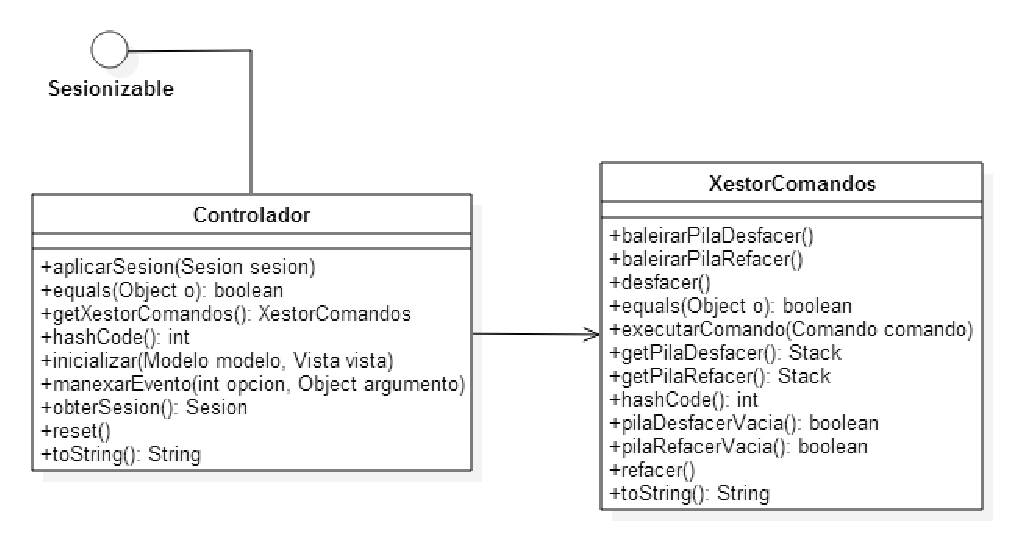
\includegraphics[width=\textwidth,height=\textheight,keepaspectratio]{figuras/UMLcontrolador}
\caption{Diagrama de clases do controlador}
\label{UMLcontrolador}
\end{figure}

O Controlador, do mesmo xeito ca o Modelo, implementa a interface Sesionizable, que permitirá que os seus campos sexan almacenados nunha sesión para ser recuperados posteriormente. Os dous métodos que deberá implementar serán obterSesion(), que obligará ao Controlador a devolver unha SesionControlador cos datos que desea salvar, e aplicarSesion(Sesion sesion), que tratará de recuperar a sesión a partir da SesionControlador previamente obtida.

O Controlador, como motor da aplicación, contén o método inicializar, que recibe unha Vista e un Modelo para comezar a desempeñar as súas funcións. Tamén contén un método reset() que reinicia a súa actividade previa cada vez que comeza un novo experimento.

A pesar de que o Controlador recibe os eventos a través do seu método máis importante: manexarEvento(int opcion, Object argumento). Para procesalos, botará man dunha clase auxiliar chamada XestorComandos, que expoñeremos a continuación. A especificación de que eventos e argumentos pode recibir este método amósase na figura \ref{manexarEvento}. Esta especificación xa figura no código fonte como o JavaDoc do método, de forma que durante a implementación teñamos acceso áxil á especificación deste método, cando estemos configurando dende a Vista as chamadas a este método do Controlador.

\begin{figure}
\centering
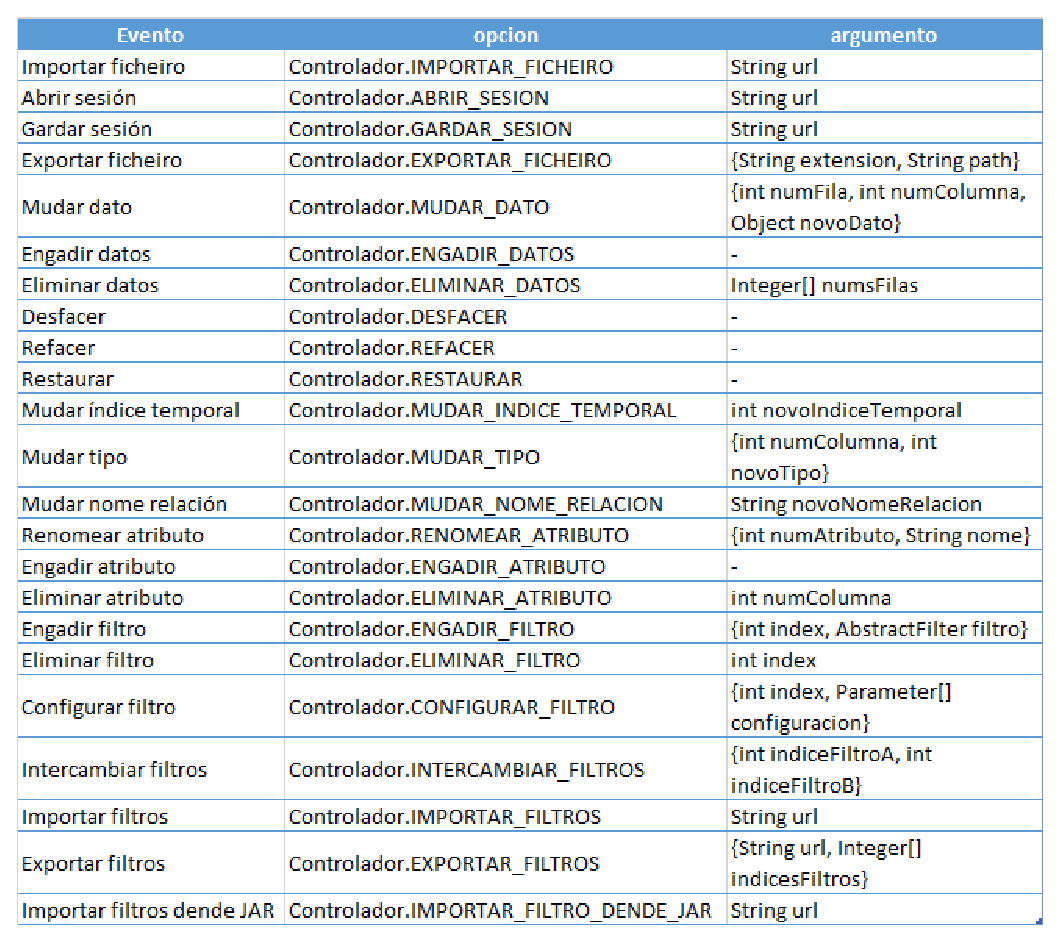
\includegraphics[width=\textwidth,height=\textheight,keepaspectratio]{figuras/manexarEvento}
\caption{Inputs do método manexarEvento}
\label{manexarEvento}
\end{figure}

O parámetro opción é un enteiro que representa ao evento, e todos os valores que pode tomar son constantes declaradas estaticamente na propia clase Controlador. O parámetro argumento debe ser de un tipo ou outro en función da opción escollida. Nos casos nos que na especificación figure unha lista de tipos entre corchetes ({String a, Integer b}), referirase a un array de obxectos ou Object[] (primeiro elemento de tipo String, segundo elemento de tipo Integer).

A clase Controlador recibe eventos a través de manexarEvento, e invoca a un método do XestorComandos para procesalo. Este método non será outro que executarComando(Comando comando). A este método o Controlador debe pasarlle unha instancia do comando que queira procesar, de xeito que a clase Controlador está traducindo eventos que recibe da Vista en comandos que envía ao XestorComandos. Entre as responsabilidades do Controlador tamén está a de recoller as excepcións que poda devolver o XestorComandos, e procesalas adecuadamente (por exemplo ordenándolle á Vista que informe do erro).

Cada vez que se termina de executar un comando, o Controlador solicita ao Modelo a execución de notifyChanged, para que en caso de que este último sufrise modificacións con motivo da execución do comando, a Vista sexa capaz de plasmar a nova información. Xuntando a relación evento-comando coa aplicación do patrón Observer conseguimos que o noso sistema se manteña sempre actualizado ante calquera cambio no Modelo, xa que a causa dos cambios debe pasar polo método manexarEvento do Controlador, e este método sempre remata chamando a notifyChanged. Ambas entidades manteranse sincronizadas sen recorrer a esperas activas ou refrescos innecesarios. Para apreciar mellor as interaccións durante todo este proceso, a figura \ref{DScomandos} contén un diagrama de secuencia que o ilustra.

\begin{figure}
\centering
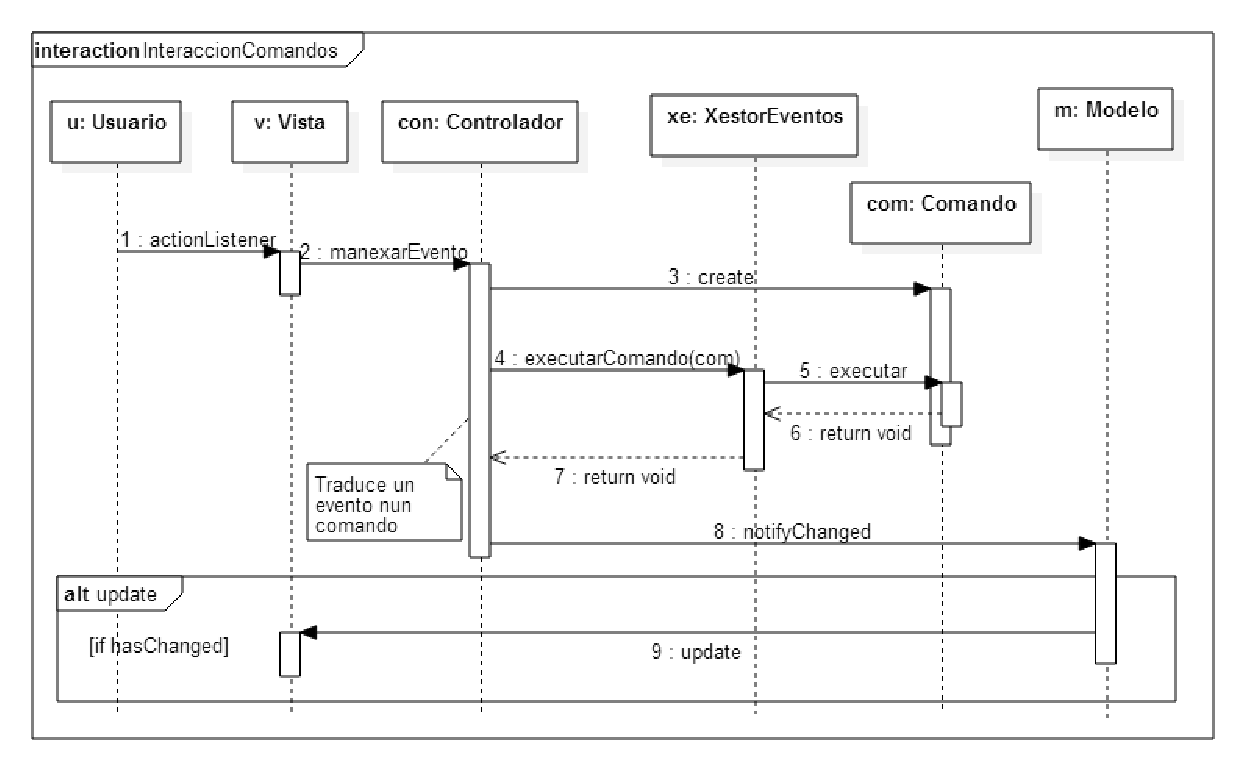
\includegraphics[width=\textwidth,height=\textheight,keepaspectratio]{figuras/DScomandos}
\caption{Diagrama de secuencia evento-notificación}
\label{DScomandos}
\end{figure}

Os comandos que o Controlador emite ao XestorComandos son a forma de manter controladas as transaccións que alteran ao Modelo. Os comandos seguen unha xerarquía que se expón na figura \ref{xerarquiaComandos}.

\begin{figure}
\centering
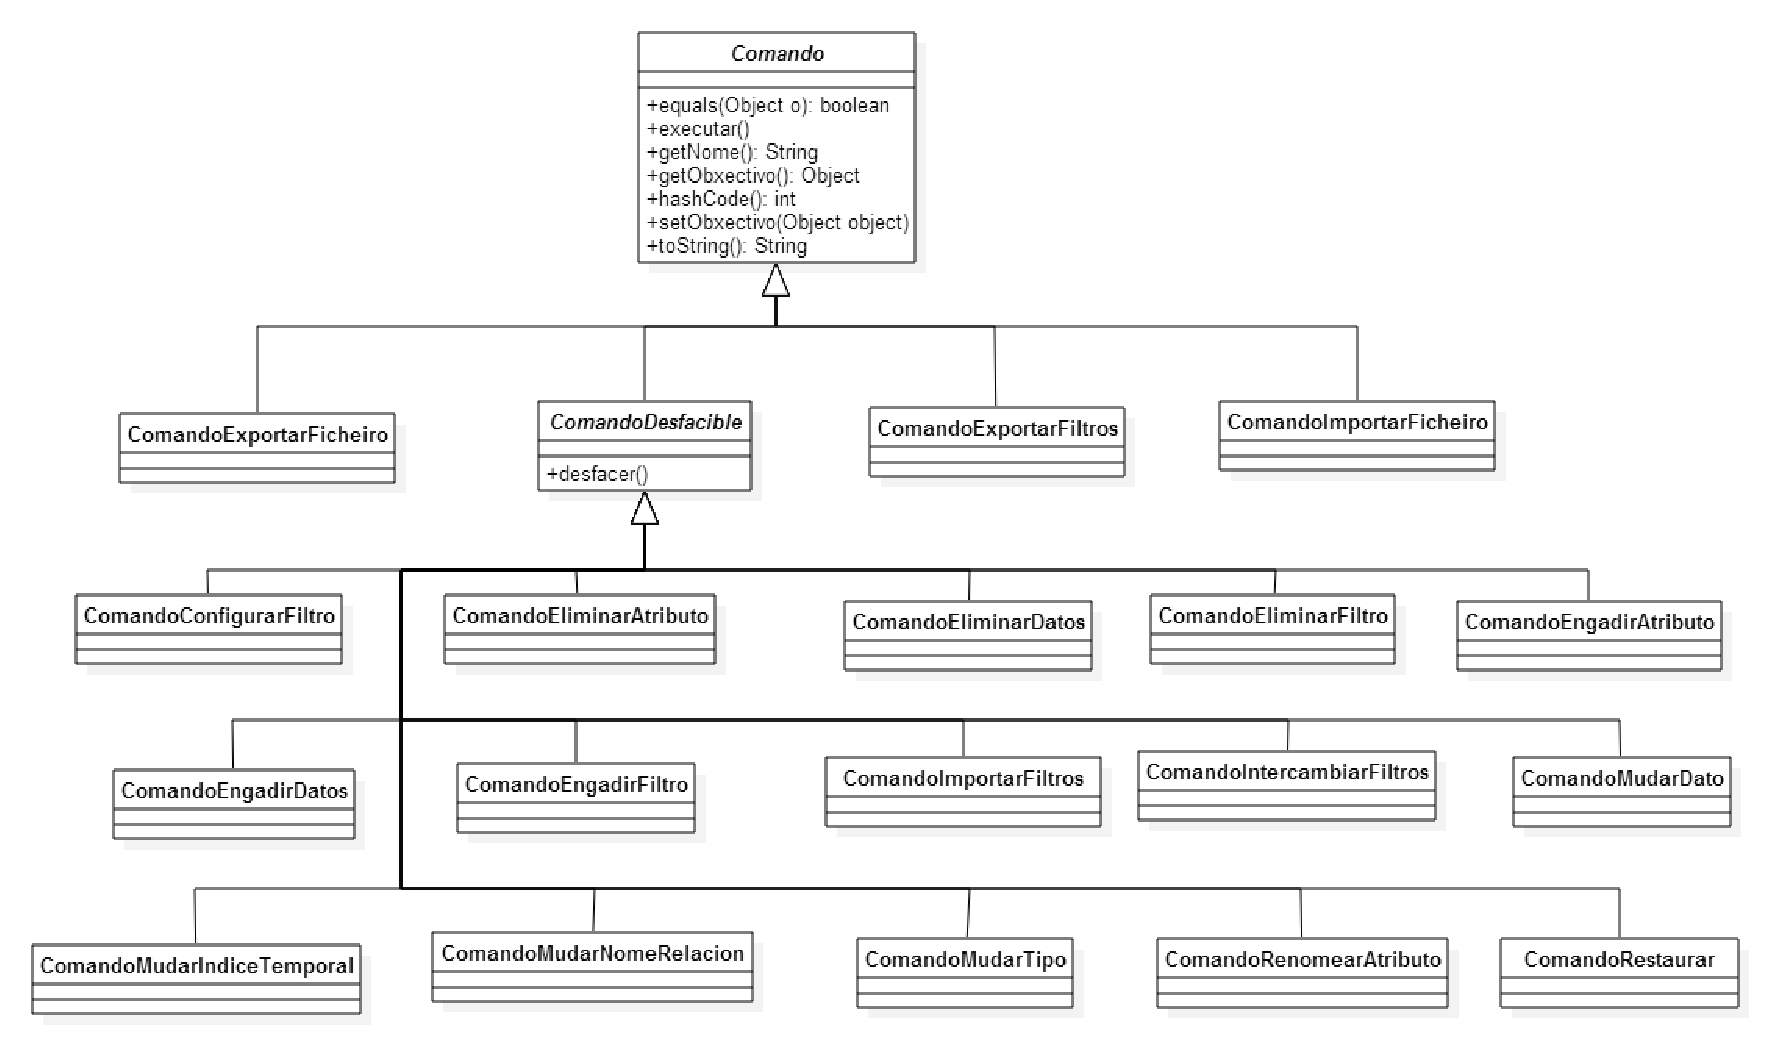
\includegraphics[width=\textwidth,height=\textheight,keepaspectratio]{figuras/xerarquiaComandos}
\caption{Xerarquía de comandos}
\label{xerarquiaComandos}
\end{figure}

Todos os comandos realizan a súa función no método executar(). O construtor da superclase Comando sempre debe recibir un Modelo (ao que tratará co nome de obxectivo). Este obxectivo, que poderemos recuperar por medio de getObxectivo(), é o que se terá que modificar no método executar(). O outro parámetro que debe recibir o construtor de Comando é o nome do comando en cuestión, que poderemos recuperar por medio de getNome().

A maioría de Comandos que o Controlador pode elixir para pasarlle ao XestorComandos son clases que estenderán a superclase ComandoDesfacible. Cando un XestorComandos recibe un Comando que deriva de ComandoDesfacible, almacenarao na pila de desfacer tras a súa correcta execución. Deste xeito, si o Controlador recibe un evento solicitando desfacer o último comando, executará o método desfacer() do XestorComandos directamente. Análogamente poderanse refacer comandos desfeitos. Cabe destacar que os eventos Desfacer e Refacer non xeran comando algún, se non que se tratan chamando ao método desfacer() ou refacer() directamente. O diagrama de secuencia destes dous eventos podémolo observar na figura \ref{xerarquiaComandos}.

\begin{figure}
\centering
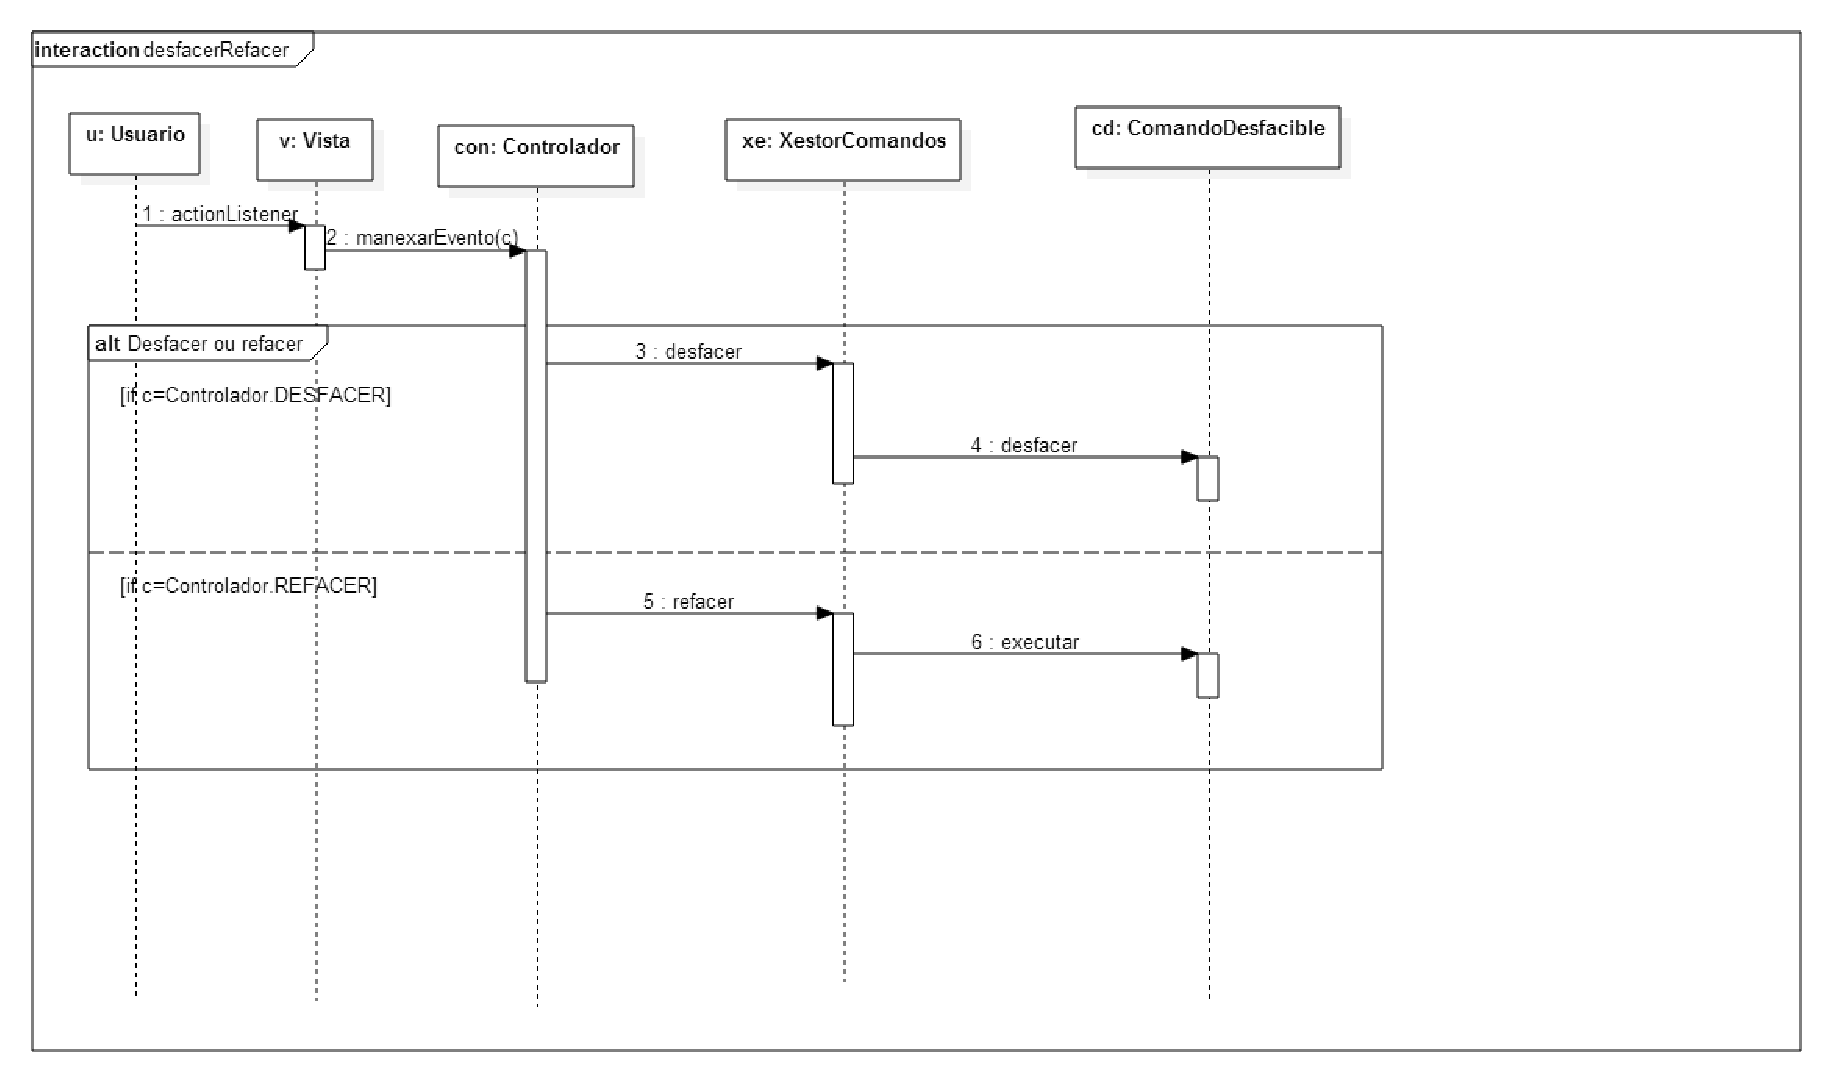
\includegraphics[width=\textwidth,height=\textheight,keepaspectratio]{figuras/desfacerRefacer}
\caption{Diagrama de secuencia dos eventos desfacer e refacer}
\label{desfacerRefacer}
\end{figure}

Do mesmo xeito que se debe implementar o método executar() para todos os comandos atendendo ao seu propósito, no caso dos ComandosDesfacibles tamén debemos implementar o método desfacer(), otorgándolle a este un comportamento que permita inverter os efectos do método executar(). A coherencia entre os procedementos executar() e desfacer() é unha responsabilidade á hora de programar comandos útiles para JDataMotion.

Existe un último grupo de comandos que comentar, e é aquel composto por comandos que aínda que estenden a clase Comando, non estenden a clase ComandoDesfacible. Estes comandos son executados sen posibilidade de entrar ou saír das pilas pilaDesfacer ou pilaRefacer que contén o XestorComandos. Trátase dos seguintes comandos:

\begin{description}

\item[ComandoExportarFicheiro:]

A exportación dun experimento supón a creación dun novo ficheiro no sistema. Esta acción non debe poder desfacerse, xa que atentaría contra a propia finalidade do comando, que é a de salvar permanentemente os datos do experimento no disco duro.

\item[ComandoExportarFiltros:]

Baixo a mesma filosofía anterior, os accesos a disco carecen da necesidade de ser reversibles.

\item[ComandoImportarFicheiro:]

O inicio dun novo experimento reinicia por completo os datos do sistema. Non se deben manter as pilas do XestorComandos dun experimento a outro.

\end{description}

\subsection{Vista}

A continuación expoñeremos e comentaremos o deseño da sección Vista. O diagrama de clases preséntase na figura \ref{UMLvista}. A Vista é

\subsubsection{Deseño da interface gráfica}

Nesta sección configuraremos o deseño da interface gráfica. A Vista é a clase encargada de darlle soporte, delegando certas funcións ou responsabilidades en clases propias asociadas ou internas. Para o deseño da aplicación gráfica teremos en conta as posibilidades da librería gráfica Swing de Java, así como os elementos ou gadgets que a compoñen. 

A utilidade da ferramenta radica no seu uso secuencial: comezamos o noso traballo a partir dun ficheiro (de datos ou de sesión) para revisar os datos e incluso formatealos ou editalos, opcionalmente aplicamos algún filtro global que afecte a todos os campos dunha determinada columna e finalmente visualizamos o resultado. A interface pode colaborar a que este proceso sexa intuitivo, de xeito que dividiremos a interface en tres seccións, ás que se accederá a través de lapelas (o gadget JTabbedPane permitiranos traballar cos 3 contedores de xeito separado). Estas seccións son:

\begin{description}
\item[Modelo:] conterá unha táboa na que cada columna representará un dos atributos, e cada fila unha instancia que pode conter valores para cada un desos atributos. As instancias á sua esquerda unha columna adicional e non editable que indique o índice da instancia. Á dereita da táboa reservaremos un espacio para arroxar información sobre un atributo ao seleccionalo. Por exemplo, ao seleccionar un atributo de tipo numérico (pulsando na cabeceira da columna que o representa) indicarase neste espacio á dereita a media de valores, o máximo, o mínimo, a desviación típica, etc. O mockup desta sección pódese observar na figura \ref{Modelo}.
\begin{figure}
\centering
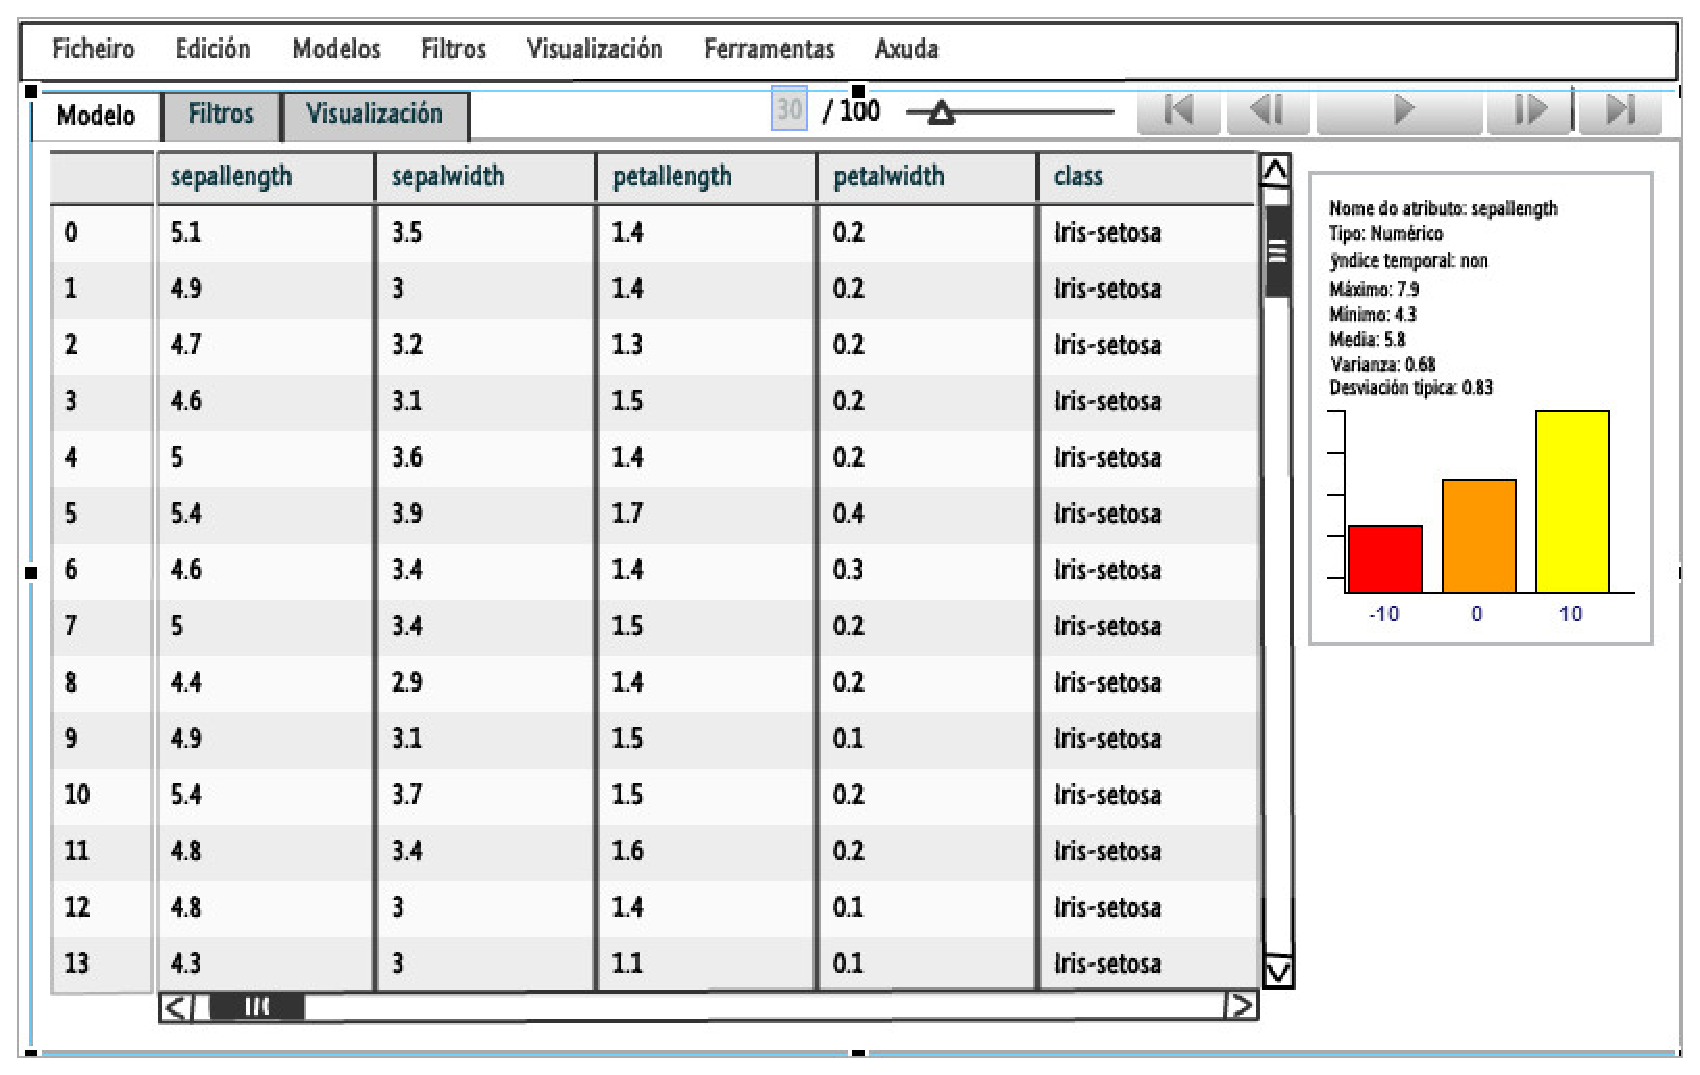
\includegraphics[width=\textwidth,height=\textheight,keepaspectratio]{figuras/Modelo}
\caption{Mockup da sección Modelo}
\label{Modelo}
\end{figure}
\item[Filtros:] conterá unha lista de filtros dispoñibles pegada á borde esquerda, e un botón baixo ela que se active cando haxa un filtro desta lista seleccionado, para engadilo. O resto do contedor ocuparao unha secuencia de iconas en fila, facendo referencia aos distintos filtros que se engadiron e aos modelos parciais que temos antes e despois de cada filtro. O mockup desta sección pódese observar na figura \ref{Filtros}.
\begin{figure}
\centering
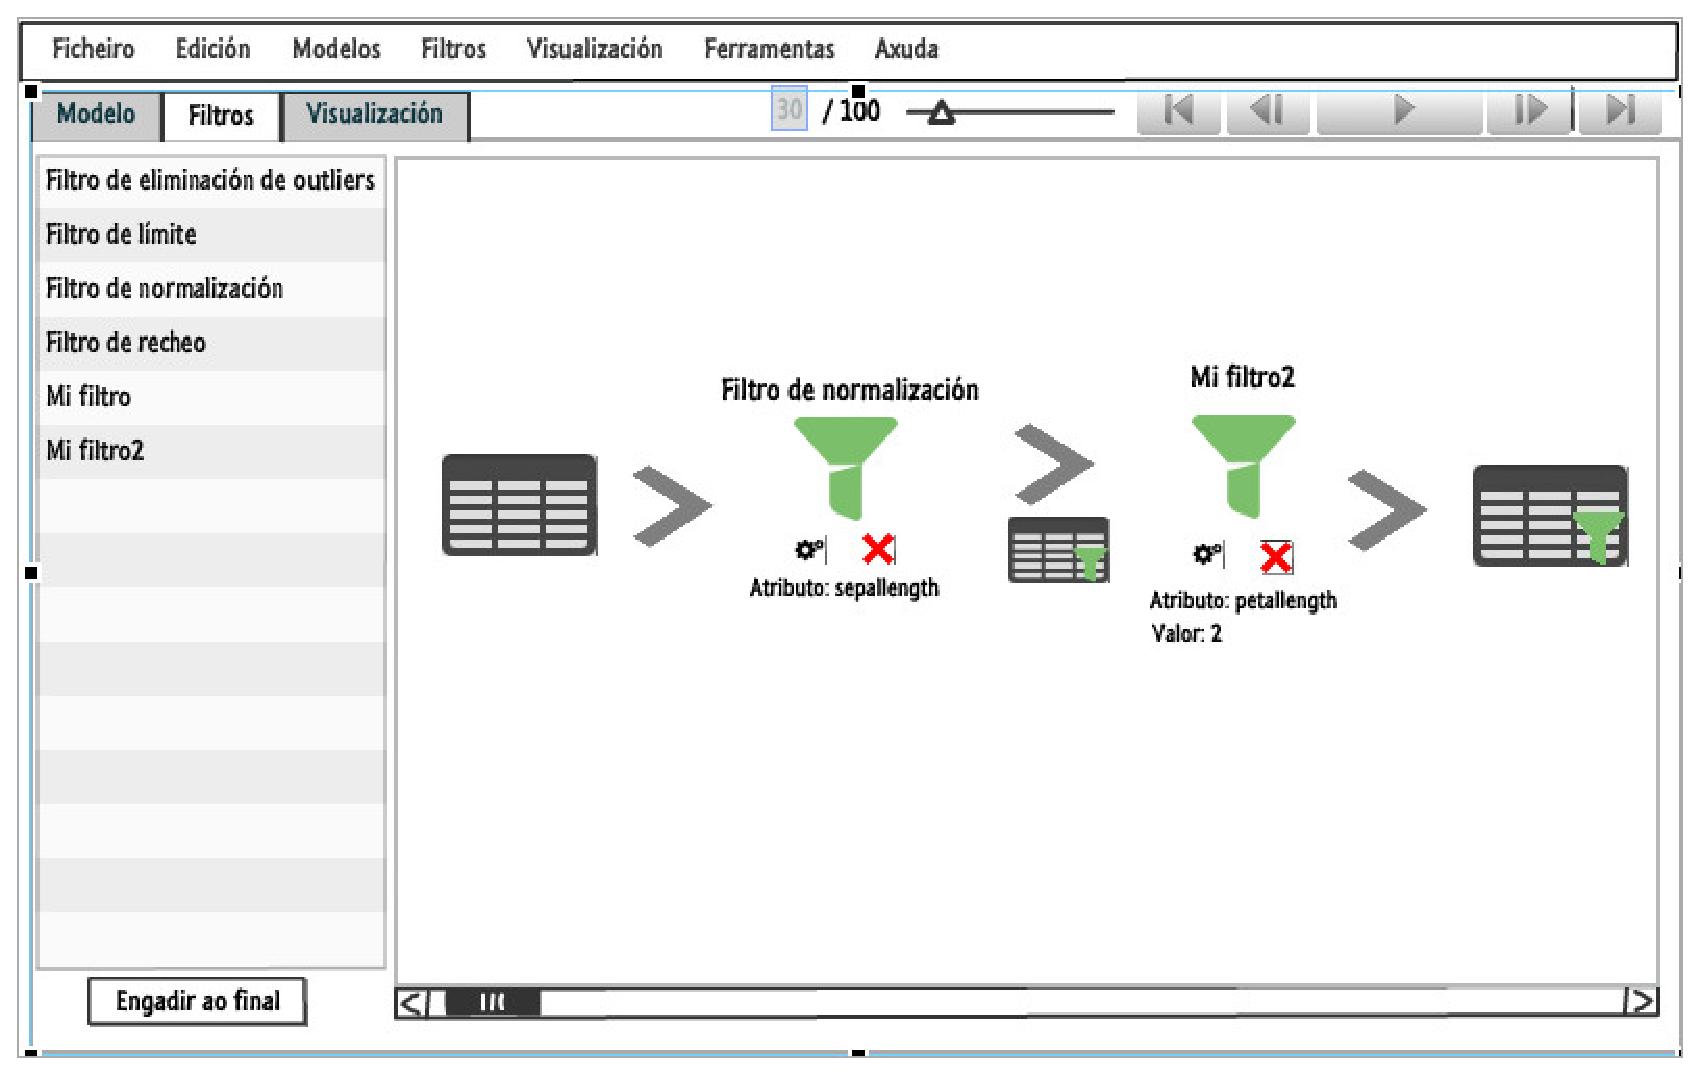
\includegraphics[width=\textwidth,height=\textheight,keepaspectratio]{figuras/Filtros}
\caption{Mockup da sección Filtros}
\label{Filtros}
\end{figure}
\item[Modelo:] a totalidade do espacio para esta sección ocuparao un conxunto de diagramas de dispersión organizados baixo unha matriz, de xeito que en cada fila da matriz os diagramas teñan o mesmo atributo para as ordenadas, e en cada columna da matriz os diagramas teñan o mesmo atributo para as abscisas. Cada diagrama disporá dun botón para ser ampliado nunha ventá aparte. Tamén figurarán dentro desta sección aínda que fora do propio contedor (en liña coas lapelas das seccións) 5 botóns asociados a funcións de reprodución (ir a principio, paso atrás, reproducir/pausar, paso adiante e ir ao final), así como un pivote desprazable ao longo dunha barra (moverase conforme se reproduza o experimento) e un indicador do número de elementos xa visualizados e totais. O mockup desta sección pódese observar na figura \ref{Visualizacion}.
\begin{figure}
\centering
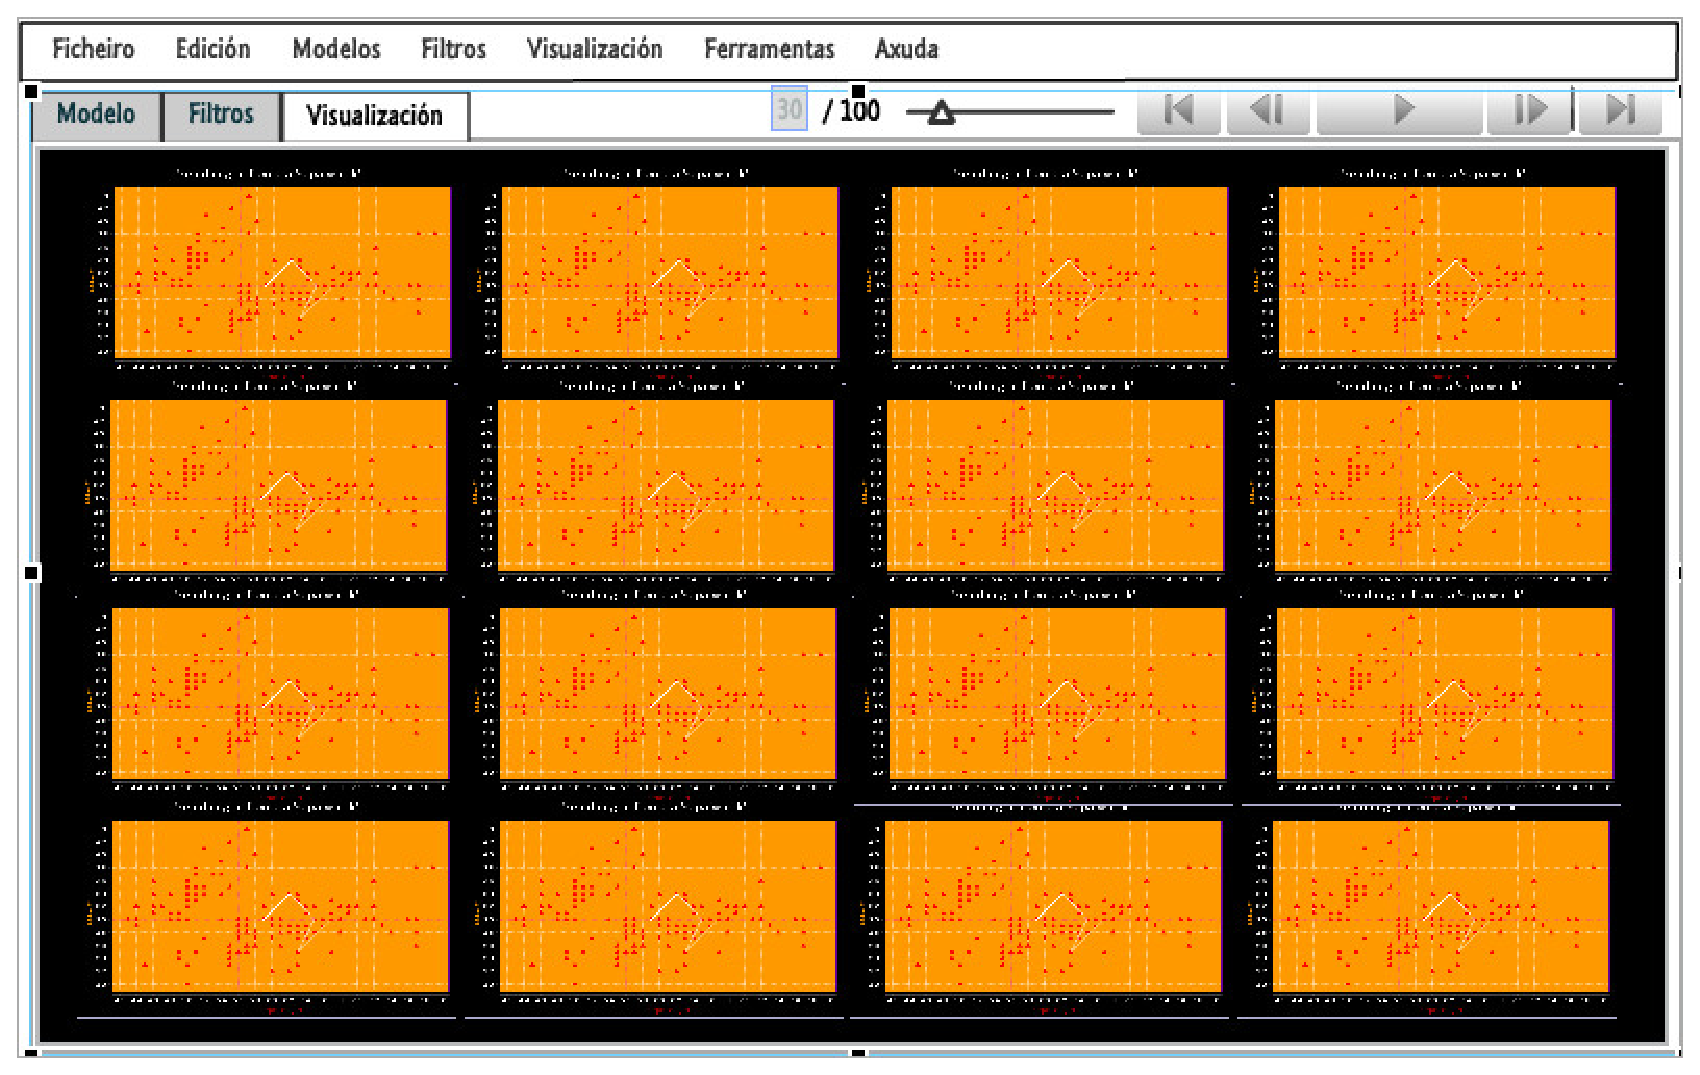
\includegraphics[width=\textwidth,height=\textheight,keepaspectratio]{figuras/Visualizacion}
\caption{Mockup da sección Visualizacion}
\label{Visualizacion}
\end{figure}
\end{description} 

Cada sección foi previamente deseñada a nivel gráfico por medio da ferramenta Lumzy, da cal acabamos de presentar algunhas capturas de pantalla. Para acceder ao mockup e ter unha mínima interacción con el (navegando a través das seccións), podemos utilizar o seguinte enlace (probado a día 10/07/2015):
\\
http://lumzy.com/access/?id=83517845D38CCEEA54A9D6B484A32147

Dada a necesidade do espacio para táboas, listas e sobre todo para a matriz de diagramas de dispersión, adoptouse a medida de desplazar os activadores de case todas as funcionalidades á barra de menús (non operativa no mockup). Prácticamente os únicos botóns que por motivos de usabilidade non podían ser desprazados cara a barra de menús eran os de funcións de reprodución, e de feito tiveron que ir encaixados fóra da propia sección de Visualización sobre a que operan. Entre outros, na barra de menús haberá un título para cada unha das 3 seccións.

Os ítems da barra de menús son os seguintes:

\begin{description}

\item[Ficheiro:] \hfill

\begin{description}

\item[Importar ficheiro:] \hfill \\
Abre unha ventá cun explorador de ficheiros para seleccionar un arquivo en formato .arff ou .csv. A dirección a ese arquivo mándase ao Controlador como argumento, acompañando a un evento de tipo IMPORTAR\_FICHEIRO.

\item[Exportar ficheiro:] \hfill \\
Abre unha ventá cun explorador de ficheiros para seleccionar unha ruta e un nome de arquivo en formato .arff ou .csv. A dirección a ese novo arquivo mándase ao Controlador como argumento, acompañando a un evento de tipo EXPORTAR\_FICHEIRO.

\item[Abrir sesión:] \hfill \\
Abre unha ventá cun explorador de ficheiros para seleccionar un arquivo en formato .jdms. A dirección a ese arquivo mándase ao Controlador como argumento, acompañando a un evento de tipo ABRIR\_SESION.

\item[Gardar sesión:] \hfill \\
Abre unha ventá cun explorador de ficheiros para seleccionar unha ruta e un nome de arquivo en formato .jdms. A dirección a ese novo arquivo mándase ao Controlador como argumento, acompañando a un evento de tipo GARDAR\_SESION.

\item[Restaurar:] \hfill \\
Envía ao Controlador un evento de tipo RESTAURAR.

\item[Pechar:] \hfill \\
Pecha a aplicación JDataMotion.

\end{description}

\item[Edición:] \hfill

\begin{description}

\item[Desfacer:] \hfill \\
Envía ao Controlador un evento de tipo DESFACER.

\item[Rafacer:] \hfill \\
Envía ao Controlador un evento de tipo REFACER.

\end{description}

\item[Modelo:] \hfill

\begin{description}

\item[Engadir instancia:] \hfill \\
Envía ao Controlador un evento de tipo ENGADIR\_DATOS.

\item[Eliminar instancias seleccionadas:] \hfill \\
Envía ao Controlador un evento de tipo ELIMINAR\_DATOS, acompañado dun array de enteiros que contén os índices das filas do Modelo que están seleccionadas.

\item[Engadir atributo:] \hfill \\
Envía ao Controlador un evento de tipo ENGADIR\_ATRIBUTO.

\item[Eliminar atributo:] Envía ao Controlador un evento de tipo ELIMINAR\_ATRIBUTO, acompañado do índice do atributo sobre o que se pulsou.

\item[Renomear atributo:] \hfill \\
Abre un diálogo para introducir o novo nome do atributo pulsado. Envía ao Controlador un evento de tipo RENOMEAR\_ATRIBUTO, acompañado dun array de obxetos co índice do atributo sobre o que se pulsou e o novo nome do atributo.

\item[Mudar nome da relación:] \hfill \\
Abre un diálogo para introducir o novo nome para a relación. Envía ao Controlador un evento de tipo MUDAR\_NOME\_RELACION, acompañado do novo nome.

\item[Amosar todas as columnas:] \hfill \\
Volve a amosar todas as columnas que se ocultaron.

\end{description}

\item[Filtros:] \hfill

\begin{description}

\item[Importar filtros:] \hfill \\
Abre unha ventá cun explorador de ficheiros para seleccionar un arquivo en formato .jdmf. A dirección a ese arquivo mándase ao Controlador como argumento, acompañando a un evento de tipo IMPORTAR\_FILTROS.

\item[Exportar filtros seleccionados:] \hfill \\
Abre unha ventá cun explorador de ficheiros para seleccionar unha ruta e un nome de arquivo en formato .jdmf. Envía ao Controlador un evento de tipo EXPORTAR\_FILTROS, acompañado dun array de obxetos coa dirección do arquivo e un array de enteiros cos índices dos filtros seleccionados.

\item[Importar filtro dende JAR:] \hfill \\
Abre unha ventá cun explorador de ficheiros para seleccionar un arquivo en formato .jar. A dirección a ese arquivo mándase ao Controlador como argumento, acompañando a un evento de tipo IMPORTAR\_FILTRO\_DENDE\_JAR.

\end{description}

\item[Visualización:] \hfill

\begin{description}

\item[Engadir ou eliminar scatterplots:] \hfill \\
Abre unha ventá cunha matriz que enfronta a todos os atributos entre si. Os diagramas de dispersión asociados que se seleccionen ou deseleccionen aparecerán ou desaparecerán da lapela de Visualización.

\item[Establecer atributo nominal representado:] \hfill \\
Abre un diálogo para seleccionar dunha lista despregable de atributos nominais cal se desexa utilizar para diferenciar os puntos nos diagramas de dispersión.

\item[Configurar reprodutor:] \hfill \\
Abre un diálogo que permite modificar a orde da reprodución, o paso e a cor e a lonxitude da estela.

\item[Calcular distancia:] \hfill \\
Abre un diálogo que permite seleccionar dous puntos da lapela de Visualización para calcular a distancia entre eles, segundo unha fórmula editable incluída no diálogo.

\end{description}

\item[Ferramentas:] \hfill

\begin{description}

\item[Idioma:] \hfill

\begin{description}

\item[Galego:] \hfill \\
Cambia o idioma da aplicación a galego (require reiniciar).

\end{description}

\begin{description}

\item[Español:] \hfill \\
Cambia o idioma da aplicación a español (require reiniciar).

\end{description}

\begin{description}

\item[Inglés:] \hfill \\
Cambia o idioma da aplicación a inglés (require reiniciar).

\end{description}

\end{description}

\item[Axuda:] \hfill

\begin{description}

\item[Acerca de:] \hfill \\
Abre un diálogo con información acerca da aplicación e o seu desenvolvemento.

\end{description}

\end{description}

E a continuación comentaremos as funcionalidades que sí se incorporaron na lapela correspondente ao seu ámbito de actuación:

\begin{description}

\item[Modelo:] \hfill

\begin{description}

\item[Botón secundario nun atributo $\rightarrow$ Tipo:] \hfill

\begin{description}

\item[Numérico:] \hfill \\
Envía ao Controlador un evento de tipo MUDAR\_TIPO, acompañado dun array de obxectos co índice do atributo sobre o que se pulsou e a constante Attribute.NUMERIC.

\item[Nominal:] \hfill \\
Envía ao Controlador un evento de tipo MUDAR\_TIPO, acompañado dun array de obxectos co índice do atributo sobre o que se pulsou e a constante Attribute.NOMINAL.

\item[String:] \hfill \\
Envía ao Controlador un evento de tipo MUDAR\_TIPO, acompañado dun array de obxectos co índice do atributo sobre o que se pulsou e a constante Attribute.STRING.

\item[Data:] \hfill \\
Envía ao Controlador un evento de tipo MUDAR\_TIPO, acompañado dun array de obxectos co índice do atributo sobre o que se pulsou e a constante Attribute.DATA.

\end{description}

\item[Botón secundario nun atributo $\rightarrow$ Índice temporal:] \hfill \\
Envía ao Controlador un evento de tipo MUDAR\_INDICE\_TEMPORAL, acompañado do índice do atributo sobre o que se pulsou.

\item[Botón secundario nun atributo $\rightarrow$ Agochar columna:] \hfill \\
Agocha a columna da táboa correspondente ao atributo no que se pulsou.

\item[Botón secundario nun histograma:] \hfill \\
Abre un menú contextual no que se pode almacenar o histograma como unha imaxe, copialo, imprimilo ou cambiarlle o zoom ou a escala.

\item[Selección por arrastre dunha área dentro do diagrama de dispersión:] \hfill \\
Reposiciona e escala o histograma para visualizar a área marcada.

\item[Tecla control + arrastre do diagrama de dispersión:] \hfill \\
Reposiciona o histograma movendo o lenzo na dirección do cursor.

\item[Roda do rato:] \hfill \\
Acerca ou afasta o zoom do histograma.

\end{description}

\item[Filtros:] \hfill

\begin{description}

\item[Botón ``Engadir ao final'':] \hfill \\
Envía ao Controlador un evento de tipo ENGADIR\_FILTRO, acompañado dun array de obxectos co índice que representa a última posición e o filtro que se seleccionou da lista.

\item[Botóns de instancias parciais/finais:] \hfill \\
Abre unha nova ventá co modelo do experimento ao aplicar os filtros ata ese punto da secuencia.

\item[Botón mover filtro á dereita:] \hfill \\
Envía ao Controlador un evento de tipo INTERCAMBIAR\_FILTROS, acompañado dun array de obxectos co índice do filtro sobre o que se pulsou este botón e o índice seguinte.

\item[Botón mover filtro á esquerda:] \hfill \\
Envía ao Controlador un evento de tipo INTERCAMBIAR\_FILTROS, acompañado dun array de obxectos co índice do filtro sobre o que se pulsou este botón e o índice anterior.

\item[Botón configurar filtro:] \hfill \\
Abre un diálogo con campos para cubrir os valores dos parámetros do filtro (o atributo sobre o que se aplica vai incluído). Envía ao Controlador un evento de tipo CONFIGURAR\_FILTRO, acompañado dun array de obxectos co índice do filtro e o array con estes novos valores.

\item[Botón eliminar filtro:] \hfill \\
Envía ao Controlador un evento de tipo ELIMINAR\_FILTRO, acompañado do índice do filtro sobre o que se pulsou este botón.

\end{description}

\item[Visualización:] \hfill

\begin{description}

\item[Botón ``Comezar visualización'':] \hfill \\
Mesmo efecto ca Visualización $\rightarrow$ Engadir ou eliminar scatterplots

\item[Desprazador:] \hfill \\
Permite moverse a distintos puntos da reprodución, chamando ao método goTo() do ManexadorScatterplots e pasándolle a fracción de tempo na que se situou o pivote do desprazador.

\item[Botón ``Ir ao comezo'':] \hfill \\
Leva á reprodución ao instante inicial, chamando ao método goTo() do ManexadorScatterplots e pasándolle o valor 0.0.

\item[Botón ``Paso atrás'':] \hfill \\
Retrocede un paso no reprodución, chamando ao método goToBefore() do ManexadorScatterplots.

\item[Botón ``Reproducir/Pausar'':] \hfill \\
Continúa a reprodución no último punto si esta se atopa parada ou pausada, chamando ao método play() do ManexadorScatterplots. Pausa a reprodución si esta está sucedendo, chamando ao método pause() do ManexadorScatterplots.

\item[Botón ``Paso adiante'':] \hfill \\
Retrocede un paso no reprodución, chamando ao método gotoNext() do ManexadorScatterplots.

\item[Botón ``Ir ao final'':] \hfill \\
Leva á reprodución ao instante inicial, chamando ao método goTo() do ManexadorScatterplots e pasándolle o valor 1.0.

\item[Botón secundario nun diagrama de dispersión:] \hfill \\
Abre un menú contextual no que se pode almacenar a imaxe, copiala, imprimila, cambiarlle o zoom ou automatizar a escala durante a reprodución.

\item[Botón secundario nun diagrama de dispersión $\rightarrow$ Propiedades:] \hfill \\
Este ítem do menú contextual abre unha ventá con opcións de configuración gráfica (colores, fontes, formas, etc.) para aplicar aos diagramas de dispersión desta sección de xeito global. As preferencias establecidas neste menú gardaranse como configuración de usuario.

\item[Selección por arrastre dunha área dentro do diagrama de dispersión:] \hfill \\
Reposiciona e escala o diagrama para visualizar a área marcada.

\item[Tecla control + arrastre do diagrama de dispersión:] \hfill \\
Reposiciona o diagrama movendo o lenzo na dirección do cursor.

\item[Roda do rato:] \hfill \\
Acerca ou afasta o zoom o diagrama de dispersión sobre o que repousa o cursor.

\end{description}

\end{description}

\section{Deseño de JDataMotion.common}

\section{Deseño de JDataMotion.filters.sample}